\documentclass[11pt]{standalone}
\usepackage[usenames]{color} %used for font color
\usepackage{amssymb} %maths
\usepackage{amsmath} %maths

\usepackage[no-math]{fontspec}
\usepackage{unicode-math}
\setmainfont{Lato}
\setmathfont{Stix Two Math}

\usepackage{pgf,xcolor}
\definecolor{itwm_blue_04}{HTML}{005A94}
\definecolor{itwm_red}{HTML}{C00000}
\definecolor{itwm_yellow}{HTML}{FFEC7F}

\usepackage{tikz}
\usetikzlibrary{shapes.misc, shadows, decorations, arrows}
\usetikzlibrary{backgrounds}
\usetikzlibrary{calc}
\usepackage{pgfplots}
\pgfplotsset{compat=newest}
\usepgfplotslibrary{fillbetween}
\usepackage{tikzpagenodes}
\usetikzlibrary{patterns}

% 0,1 x 1,2
\begin{document}
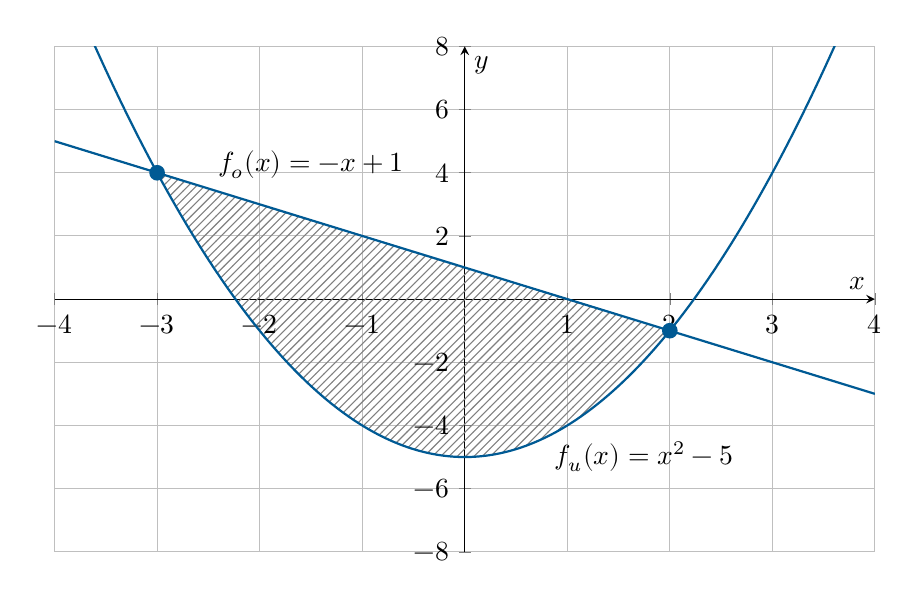
\begin{tikzpicture}
\begin{axis}[
    domain=-4:4,
    axis lines = center,
    xlabel = {$x$},
    ylabel = {$y$},
    height=8cm, width=12cm, 
    xmin=-4, xmax=4, ymin=-8, ymax=8, 
    xtick={-4, -3,...,4},
    ytick={-8, -6,...,8},
    grid = both
]
\node at (-1.5, 4.25) {$f_{o}(x)=-x+1$};
\node at (1.75, -5) {$f_{u}(x)=x^2-5$};
\addplot[draw=itwm_blue_04, samples=300, thick, name path=f]{-x+1};
\addplot[draw=itwm_blue_04, samples=300, thick, name path=g]{x^2-5};
\node[fill, itwm_blue_04, circle,inner sep=-2] at (-3,4) {};
\node[fill, itwm_blue_04, circle,inner sep=-2] at (2,-1) {};
\addplot [pattern=north east lines, pattern color=gray] fill between [of = f and g, soft clip={domain=-3:2}];
\end{axis}
\end{tikzpicture}
\end{document}